\documentclass{article}

\usepackage[english]{babel}
\usepackage{lineno, blindtext}
\usepackage[utf8]{inputenc}
\usepackage{amsmath,amssymb}
\usepackage{parskip}
\usepackage{enumitem}
\usepackage{listings}
\usepackage{graphicx}
\graphicspath{ {./images/} }
\usepackage[ruled,vlined]{algorithm2e}
%\usepackage{algorithmic}
%\usepackage{algpseudocode}

% Margins
\usepackage[top=2.5cm, left=3cm, right=3cm, bottom=4.0cm]{geometry}
% Colour table cells
\usepackage[table]{xcolor}

% Get larger line spacing in table
\newcommand{\tablespace}{\\[1.25mm]}
\newcommand\Tstrut{\rule{0pt}{2.6ex}}         % = `top' strut
\newcommand\tstrut{\rule{0pt}{2.0ex}}         % = `top' strut
\newcommand\Bstrut{\rule[-0.9ex]{0pt}{0pt}}   % = `bottom' strut

%%%%%%%%%%%%%%%%%
%   Homework 1  %
%%%%%%%%%%%%%%%%%
\title{EE 382C Multicore Computing Homework 1}
\author{
    Mitchell, Olivia\\
    \texttt{ozm59}
    \and
    Molter, Matthew\\
    \texttt{mm58286}}
\date{\today}

\begin{document}
\maketitle

%%%%%%%%%%%%%%%%%
%   Problem 1   %
%%%%%%%%%%%%%%%%%
\section{Problem 1}
 You are one of $P$ recently arrested prisoners. The warden, a deranged computer engineer, makes the following announcement:
\begin{itemize}
  \item You may meet together today and plan a strategy, but after today you will be in isolated cells and have no communication with one another.
  \item I have set up a “switch room” which contains a light switch, which is either $on$ or $off$. The switch is not connected to anything.
  \item Every now and then, I will select one prisoner at random to enter the “switch room.” This prisoner may throw the switch (from $on$ to $off$, or vice-versa), or may leave the switch unchanged. Nobody else will ever enter this room.
  \item Each prisoner will visit the switch room arbitrarily often. More precisely, for any $N$, eventually each of you will visit the switch room at least $N$ times.
  \item At any time, any of you may declare: “we have all visited the switch room at least once.” If the claim is correct, I will set you free. If the claim is incorrect, I will feed all of you to the crocodiles. Choose wisely!
\end{itemize}

\begin{enumerate}[label=\alph*)]
  \item Devise a winning strategy when you know that the initial state of the switch is $off$.
  \item Devise a winning strategy when you do not know whether the initial state of the switch is $on$ or $off$.
\end{enumerate}

\subsection{Solution 1a}

Initial State of switch is $off$.

The algorithm the prisoners should use is as follows:
\begin{itemize}[label={}]
\item Designate one prisoner to keep track of total count (lets make this prisoner $0$).
\item All the prisoners will also keep track of their own $count$ variable (which starts at $count=0$).

\item For all normal prisoners (prisoners $1$ though $N-1$):
	\begin{itemize}[label={}]
	\item When a prisoner enters the switch room:
		\begin{itemize}[label={}]
		\item if they have already flipped the switch ($count == 1$), they will immediately leave regardless of switch position.
		\item if they have not already flipped the switch ($count == 0$):
			\begin{itemize} [label={}]
			\item If the switch is set to $off$ they will flip it to $on$, set $count = 1$, and leave.
			\item If the switch is set to $on$ they will leave.
			\end{itemize}
		\end{itemize}
	\end{itemize}
\item For all the counter (prisoner $0$):
	\begin{itemize}[label={}]
	\item When counter enters the switch room:
		\begin{itemize}[label={}]
		\item If the switch is set to $on$ they will flip it to $off$, do $count++$, and leave.
		\item If the switch is set to $off$ they will leave.
		\end{itemize}
	\item If $count == N-1$, they will declare that every prisoner has been in the switch room at least once.
	\end{itemize}
\end{itemize}
This works since every prisoner will set the switch to $on$ only once and there is a prisoner keeping track of the total counts of the switch being set to $on$. 

\subsection{Solution 1b}

Initial state of switch could be $on$ or $off$.

The algorithm the prisoners should use is as follows:
\begin{itemize}[label={}]
\item Designate one prisoner to keep track of total count (lets make this prisoner 0).
\item All the prisoners will also keep track of their own $count$ variable (which starts at $count=0$).

\item For all normal prisoners (prisoner $1$ though $N-1$):
	\begin{itemize}[label={}]
	\item When a prisoner enters the switch room:
		\begin{itemize}[label={}]
		\item If they have already flipped the switch twice ($count == 2$), they will immediately leave regardless of switch position.
		\item If they have not already flipped the switch twice ($count < 2$): 
			\begin{itemize}[label={}]
			\item if the switch is set to $off$ they will flip it to $on$, do $count++$, and leave.
			\item if the switch is set to $on$ they will leave.
			\end{itemize}
		\end{itemize}
	\end{itemize}
\item For all the counter (prisoner $0$):
	\begin{itemize}[label={}]
	\item When counter enters the switch room:
		\begin{itemize}[label={}]
		\item If the switch is set to $on$ they will flip it to $off$, do $count++$, and leave.
		\item If the switch is set to $off$ they will leave.
		\end{itemize}
	\item If $count == 2(N-1)$, they will declare that every prisoner has been in the switch room at least once.	
	\end{itemize}
\end{itemize}
This works since at most every prisoner will set the switch to $on$ twice and every prisoner will set the switch at least once (in the case that the switch is initialized to $on$ one prisoner will have only set the switch once).   

%%%%%%%%%%%%%%%%%
%   Problem 2   %
%%%%%%%%%%%%%%%%%
\pagebreak
\section{Problem 2}
Show that any of the following modifications to Peterson’s algorithm makes it incorrect:

\begin{enumerate}[label=\alph*)]
  \item A process in Peterson’s algorithm sets the $turn$ variable to itself instead of setting it to the other process.
  \item A process sets the turn variable before setting the $wantCS$ variable.
\end{enumerate}


\subsection{Solution 2a}
Take the following possible order of executions.

\begin{linenumbers}
	wantCS[0] = true;
	
	wantCS[1] = true;
	
	turn = 0; // $P_0$ enters CS since $P_1$ does not yet want to enter the CS.
	
	turn = 1; // $P_1$ enters CS. $P_0$ is already in the CS, but it is not $P_0$'s turn.
\end{linenumbers}

It can be seen that it is possible for both processes can enter the critical section at the same time. This violates mutual exclusion.

\subsection{Solution 2b}
Take the following possible order of executions.

\begin{linenumbers}
	turn = 1;
	
	turn = 0;
	
	wantCS[1] = true; // $P_1$ enters CS. It is $P_0$'s turn, but it does not want the CS.
	
	wantsCS[0] = true; // $P_0$ enters CS. $P_1$ is already in the CS, but it is not $P_1$'s turn.
\end{linenumbers}

It can be seen that it is possible for both processes can enter the critical section at the same time. This violates mutual exclusion.


%%%%%%%%%%%%%%%%%
%   Problem 3   %
%%%%%%%%%%%%%%%%%
\pagebreak
\section{Problem 3}
The $l-exclusion$ problem is a variant of the starvation-free mutual exclusion problem. We make two changes: as many as $l$ threads may be in the critical section at the same time, and fewer than $l$ threads might fail (by halting) in the critical section. An implementation must satisfy the following conditions:

\begin{description}[font=\scshape\bfseries]
\item [$l-Exclusion$:] At any time, at most $l$ threads are in the critical section.
\item [$l-Starvation-Freedom$:] As long as fewer than $l$ threads are in the critical section then some thread that wants to enter the critical section will eventually succeed (even if some threads in the critical section have halted).
\end{description}

Modify the $n$-process $Filter$ mutual exclusion algorithm to turn it into an $l-exclusion$ algorithm.

\subsection{Solution 3}
Solving for $l-exclusion$ requires that we add an integer variable for $l$, and each process must ensure that less than $l$ processes are in the critical section, or ahead of it in the wait for the critical section before entering. This is done by checking all processes for gates they are trying to enter, and each process attempting to access a gate higher than the current thread is ahead of it in line. If after the check, fewer than $l$ processes are in the CS or ahead in line, the current process enters the CS.

Modified algorithm:

\begin{lstlisting}
defn:
int N; // number of processes
int L; // number of processes allowed to access CS simultaneously
int[] gate; // for thread i, gate[i] stores gate thread i is trying to enter; init 0s
int[] last; // for gate k, last[k] stores last thread id trying to enter; init 0s

requestCS(int i):
	for(int k = 1; k < N - L + 1; k++) {
		gate[i] = k;
		last[k] = i;
		int ahead = L+1;

		//while I am not at the head of the wait line and I am the last person 
		//to enter this gate/waiting room
		while(ahead > L && last[k] == i) {
			ahead = 0;
				
			//look at all the processes and if they are ahead of me in line, 
			//update the ahead counter
			for (int m = 0; m < N; m++) {
				if(gate[m] >= k) {
					ahead++;
				}//end if
			}//end for
		}//end while
		 //less than L processes are in the CS and ahead in line, or another
		 //process has tried to enter the same gate
		 //either way, move to the next gate
	}//end for
	
releaseCS(int i):
	// remove myself from the wait queue
	gate[i] = 0;

\end{lstlisting}

%%%%%%%%%%%%%%%%%
%   Problem 4   %
%%%%%%%%%%%%%%%%%
\pagebreak
\section{Problem 4}
Write a Java class that computes frequency of an item in an array of integers. It provides the following $static$ method:

%Java code
\begin{lstlisting}[language=Java]
public class Frequency {
  public static int parallelFreq(int x, int[] A, int numThreads) {
    // your implementation goes here.
  }
}
\end{lstlisting}

This method creates as many threads as specified by $numThreads$, divides the array $A$ into that many parts, and gives each thread a part of the array. Each thread computes the frequency of $x$ in its own subarray in parallel. The method should return the overall sum of the frequencies. Use $Callable$ interface for your implementation.

%%%%%%%%%%%%%%%%%
%   Problem 5   %
%%%%%%%%%%%%%%%%%
\pagebreak
\section{Problem 5}
Write a program that uses $n$ threads, where $n = 1..8$. These threads increment a shared variable $c$. The total number of increment operations are $m = 1, 200, 000$. Each thread reads the value of $c$ and increments it $m/n$ times. Implement the following methods and compare the the total time taken for each of
the following methods for $n = 1..8$.

%Java code
\begin{lstlisting}[language=Java]
public class PIncrement {
  public static int parallelIncrement(int c, int numThreads) {
    // your implementation goes here
  }
}
\end{lstlisting}


Submit the plot as part of the assignment.

\begin{enumerate}[label=\alph*)]
  \item Peterson’s Tournament Algorithm.
  \item Java’s AtomicInteger (with $compareAndSet$ method)
  \item Java’s synchronized construct
  \item Java’s Reentrant Lock
\end{enumerate}

Remember to use $volatile$ qualifier for shared variables to guarantee
atomicity for part (a).

\subsection{Plot of average of 100 run times of each method over number of threads}
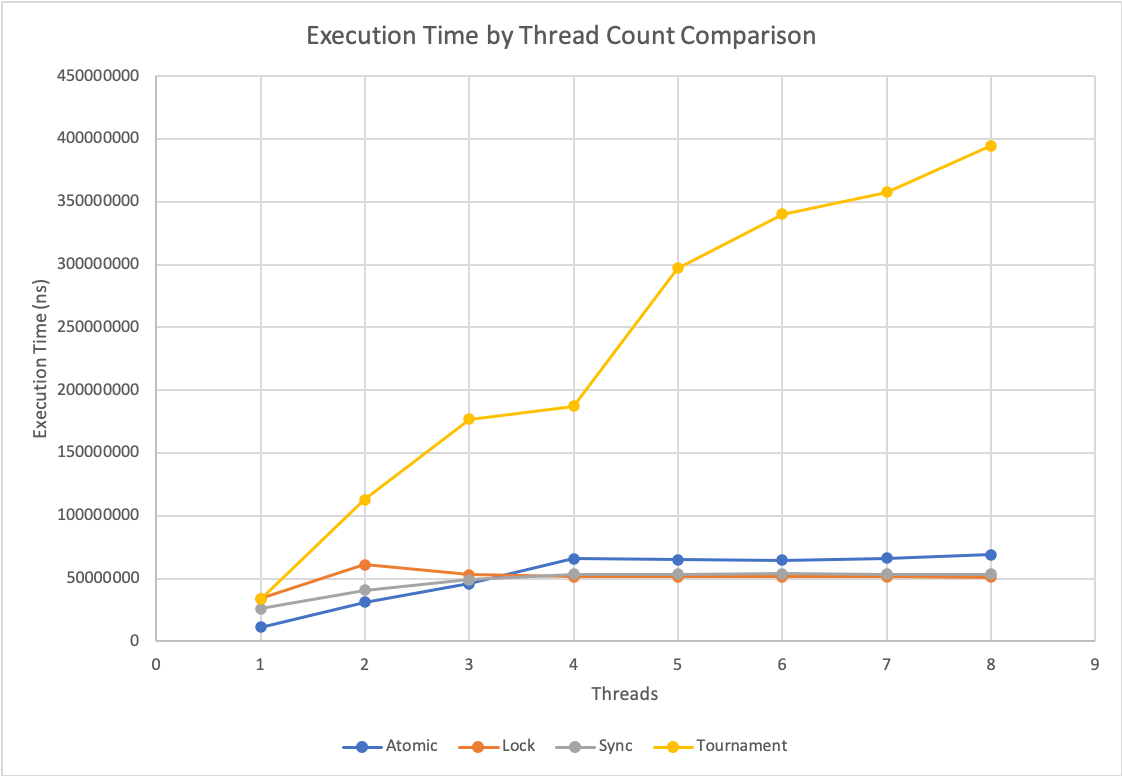
\includegraphics[width=12cm]{aggregate}

\subsection{Note on Tournament Implementation}
Since it is impossible to make an array of $volatile$ data types (the $volatile$ ends up becoming attached to the array pointer instead), arrays of AtomicBooleans were used for the $want$ and $turn$ arrays. The only way to allocate arrays of $volatile$ booleans would be to implement a JAVA class encapsulating a single $volatile$ boolean which would be a simple version of AtomicBoolean.

\subsection{Data Trends}
Tournament, to no huge surprise, performs the worst of the four methods. Its performance increases most dramatically when a level is added to the tournament (between thread counts: 2 to 3, and 4 to 5). Atomic performs best at lower thread counts (1 though 3) and lock performs best on the higher number of threads (5 though 8). What is surprising is that as threads increase sync, lock, and atomic jump up in time period and then the time decreases until the next jump up. Perhaps, like in Tournament, the implementation has to do significantly more work/allocate more resources at certain intervals.  

\end{document}
